\section{Structural Health Monitoring}

\subsection{Definition}

According to  \citet{balageas2010}, the \gls*{shm} main purpose is to provide, during the life of a structure,  a diagnosis of: the state of the constituent material; the different parts of the structure; and the full assembly of each part that makes the structure as a whole. 
It is an improved way to make non-destructive evaluation.
It can be applied in several areas such as civil infrastructure, like bridges and buildings; aerospace, like airplanes and spaceships; and mechanical, like machines.

% \begin{figure}[H]
%     \centering
%     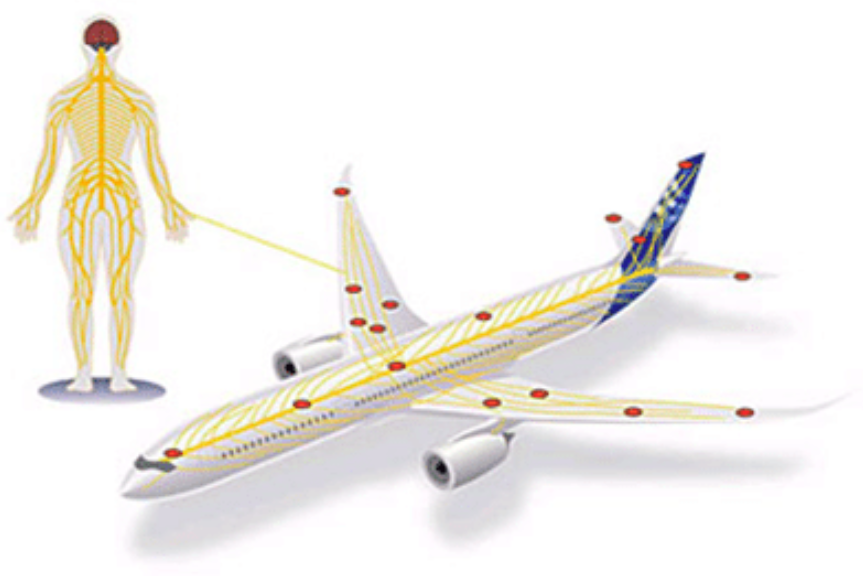
\includegraphics[width=0.6\textwidth]{figures/2methodology/shm/smh_nervous_system.png}
%     \caption[SHM and human nervous system analogy]{\gls*{shm} and human nervous system analogy. Source: \citet{blanckenstein2015}}
%     \label{fig:shm_nervous_system}
% \end{figure}

Furthermore, it also can be associated as an analogy to the human nervous system. Just like the sensors send a signal to the central processor, the human 
senses send a signal to the brain to make the recognition of what is happening.

\subsection{Brief History}

The \gls*{shm} development began back in the 20th century and it has been coupled with the evolution of the digital computing hardware, what allowed the costs of the applied techniques less expensive over time.

It all starts back in the early 1970s and 1980s. 
The oil industry tried to develop vibration-based damage identification methods for offshore platforms by simulating damage scenarios, examining the changes in the resonant frequencies and correlating them with those measured on a platform.
In the same period, the aerospace community studied vibration-based damage identification along with the development of the space shuttle. 
From that, it was developed the shuttle modal inspection system which aimed to identify fatigue damage in components like fuselage panels and control surfaces. The system was so successful that all orbiter vehicles had been periodically subjected to this test.
Also, the civil engineering community studied vibration-based damage evaluation of bridge structures and buildings in the late 1980s \citep{farrar2007}.

From the late 1990s to the early 2000s, \citet{sohn2003} showed the evolution of the techniques used in \gls*{shm}, analyzing mainly the following factors: the operational evaluation; data acquisition and cleansing; feature extraction; and statistical modeling for feature discrimination. 
He also verified that the statistical patter recognition had not been embraced by the researchers to be more often used in such matter.

Nowadays, in order to contour inherent issues of \gls*{shm} methods, as large computational effort and hand-crafted work that results in poor classification performance, many deep learning techniques have been used, such as \gls*{cnn} \citep{avci2017}.

\subsection{Main Techniques}

\subsubsection*{Accelerometers}

The use of accelerometers is consolidated in the engineering community to be used in several areas and it is present in the people daily life in things like game consoles, smartphones, and tablets.

\gls*{mems} sensor have several applications in measuring linear acceleration or angular motion along axis as an input to control a system.
\gls*{mems} accelerometer sensors often measure the movement of a mass with a position-measuring interface circuit that is converted into a digital electrical signal by an analog-to-digital converter for digital processing \citep{dadafshar2014}.

In \gls*{shm} situation, the accelerometers are in the \gls*{mems}. The \gls*{mems} are, then, embedded in the structure and can provide information about the structure by detecting low-amplitude and low-frequency vibrations that are not always viable with the conventional low-cost sensor boards \citep{sabato2017}.

There are many others sensors used in vibration-base techniques like velocity and displacement sensors, however the accelerometers are widely used for this purpose.

\subsubsection*{Piezoelectric materials}

When dealing with acoustic-based techniques, the use of piezoelectric materials as sensor is a great choice due to its ability to respond to stimuli, incorporation, and compatibility with construction materials. Beyond that, these materials are relatively cost-efficient and can sense vibrations in the structures they are installed \citep{jiao2020}.

Piezoelectric materials and their main property were discovered back in 1880 \citep{curie1880}. 
The phenomenon is that by the application of pressure in those kinds of materials in the correct direction, it is observed the production of a potential difference and consequently an electrical charge. 
Examples of materials that are piezoelectric are quartz, zinc, sodium chlorate, tourmaline, calamine, topaz, tartaric acid, cane sugar, and others \citep{brown1962}.

The application of these materials in \gls*{shm} is basically to install the piezoelectric sensor in the structure intend to be monitored and through the tension or compression in it done, a sign will be sent to the central system by the potential differential. 
The signal indicates that something not usual is happening in the structure. Of course there are levels of the signals and each case must be evaluated in its context. 
In the last years the use of piezoelectric materials has been capable to identify failures, like the presence of delamination damage, as long as the piezoelectric sensors are close to the damage \citep{maio2011}.

\subsubsection*{Optical-based} %  digital image correlation

The use of digital cameras to detect any kind of irregularity in the surface is also a way to monitor the structure, mainly in the surface areas. The camera itself may be static in a strategical position that allow it to provide good images to be analyzed or can be embedded in the structure itself or in an \gls*{uav} that will surround it.

To automate and improve the accuracy of the damage detection, image processing techniques are employed, that being a non-conventional approach \citep{sharma2016}. In the civil engineering context, it is commonly utilized computer vision to damage detection \citep{feng2018} and also \gls*{uav} integrated in the same local as the structures for \gls*{shm} \citep{sankarasrinivasan2015}.

Many of the images obtained can have their not only the images improved by \gls*{ai}, but also the analyses can take advantage of it.

\subsection{Railway}

\subsection{SHM and Crack Detection on Railway}